% Staircase paper for 18.821 Fall 2012 project 3.
% Authors: Daniel Grazian, Michael Mekonnen, Agustin O Venezuela III

\documentclass[12pt]{amsart}

% Keep everything here in alphabetical order, please! :) -jven

% Packages

\usepackage{amssymb}
\usepackage{graphicx}

% Enumeration

\newtheorem{theorem}{Theorem}[section]

\newtheorem{conjecture}[theorem]{Conjecture}
\newtheorem{corollary}[theorem]{Corollary}
\newtheorem{definition}[theorem]{Definition}
\newtheorem{example}[theorem]{Example}
\newtheorem{examples}[theorem]{Examples}
\newtheorem{lemma}[theorem]{Lemma}
\newtheorem{proposition}[theorem]{Proposition}
\newtheorem{remarks}[theorem]{Remarks}
\newtheorem{remark}[theorem]{Remark}

% Utility commands
% Real numbers
\newcommand{\R}{\mathbb{R}}
% Figures: \newfigure{label}{caption}{content}
\newcommand{\newfigure}[3]{
\begin{figure}
#3
\caption{#2 \label{#1}}
\end{figure}
}
% Sections: \newsection{title}{label}
\newcommand{\newsection}[2]{
\section{#1 \label{#2}}
}

\title{A Staircase Model of Erosion}
\author{Daniel Grazian, Michael Mekonnen, Agustin O Venezuela III}
\date{November 3, 2012}

\begin{document}

\begin{abstract}
TODO(dgrazian, jven, mikemeko)
\end{abstract}

\maketitle

\newsection{Introduction}{sec:intro}
In this paper, we consider the random process of forming staircases by dropping blocks into an infinite row of infinitely tall columns.

More concretely, consider partitioning the first quadrant of $\R^2$ into axis-aligned columns of width $1$, as in Figure $\ref{fig:columns}$. We will index the columns starting at $0$.

\newfigure{fig:columns}{Partitioning of the first quadrant into columns}{
BLAH
}

Now consider iteratively placing unit squares (blocks) into these columns. We will say that a block is at location $(i, j)$ for non-negative integers $i, j$ if it is axis-aligned and its bottom-left vertex is at $(i, j)$. At each step, a block can be placed at $(i, j)$ if and only if (1) $i = 0$ or there is a block at $(i - 1, j)$ and (2) $j = 0$ or there is a block at $(i, j - 1)$. Figure $\ref{fig:dropblocks}$ shows an example of a valid sequence of placing $5$ blocks. We will usually refer to such a sequence of placements a \textit{dropping of $5$ blocks}, for obvious reasons. We call a configuration of $n$ blocks in the first quadrant a \textit{staircase} if it can be obtained by dropping $n$ blocks.

\newfigure{fig:dropblocks}{Example of dropping $5$ blocks}{
SUP
}

We will refer to a staircase as the monotonically decreasing finite sequence of positive integers $(b_i)$, where $b_i$ is the number of blocks in column $i$. For example, the last staircase in Figure \ref{fig:dropblocks} can be written as $(hi,hi,hi,hi,hi)$. Note that we do not include columns that do not contain any blocks.

We are interested in constructing random staircases: beginning with no blocks, we consider all the locations $(i, j)$ at which a block can be validly placed, choose such a location uniformly at random, and place a block there. This raises various interesting questions regarding the distribution over the shape of the resulting staircase when $n$ blocks are dropped.

To begin, Section \ref{sec:numstaircases} will address the question of how many staircases exist with $n$ blocks. Section \ref{sec:expectedcolumns} will present numerical results for the expected number of columns for a staircase with $n$ blocks. Finally, Section \ref{sec:twocolumn} will present exact results for the variant of the problem in which we restrict staircases to having at most $2$ columns.

\newsection{Number of Staircases with $n$ Blocks}{sec:numstaircases}
Our investigation into the distribution over staircase shapes begins with determining how many staircase shapes exist using $n$ blocks.

\begin{theorem}
The number of staircases with $n$ blocks is equal to the number of partitions of $n$ (the number of ways to write $n$ as a sum of positive integers, irrespective of the order of the parts).
\begin{proof}
There is an obvious bijection $f$ between staircase with $n$ blocks and partitions of $n$. We map the staircase $(b_i)$ with $n$ blocks to the partition $n=\sum b_i$.

$f$ is injective. If $(b_i)\neq (b_i')$ are two distinct staircases, then $n = \sum b_i = \sum b_i'$ are two partitions of $n$ such that with the parts written in monotonically decreasing order, we have some $b_i\neq b_i'$. It follows that the two partitions are distinct.

$f$ is also surjective. Given a partition $n = \sum a_i$, we can sort $(a_i)$ in monotonically decreasing order, yielding $(b_i)$. $f$ clearly maps $(b_i)$ to the partition $\sum a_i$.

The result follows.
\end{proof}
\end{theorem}

For increasing $n$ beginning with $n = 0$, the numbers of partitions of $n$ are $1, 1, 2, 3, 5, 7, 11, \ldots$. Unfortunately, this sequence is known to grow exponentially with $n$: for $n = 100$, there are $190,569,292$ partitions. This appears to make our original goal of finding a distribution over staircase shapes difficult as there are exponentially many objects to which a probability is to be assigned. For this reason, we instead consider the distribution over the number of columns in the next section, the number of which is clearly linear in $n$.

\newsection{Expected Number of Columns}{sec:expectedcolumns}
TODO(dgrazian)

\newsection{2-Column Staircases}{sec:twocolumn}
\section{$2$-Column Staircases\label{sec:2column}}
TODO(mikemeko): update section based on what we choose to use to denote a particular staircase
Now we restrict ourselves to staircases of the form $(m,n)$ that have at most $2$ columns. We are interested in finding the number of ways to construct the $(m,n)$ staircase.

\begin{definition}
Let $T(m,n)$ denote the number of different ways to construct the $(m,n)$ staircase.
\end{definition}

We start by writing a recurrence to describe $T(m,n)$:
\begin{equation}
T(m,n) = \left\{ 
  \begin{array}{l l}
    T(m-1,n) + T(m,n-1) & \quad \text{if $m \geq n > 0$}\\
    1 & \quad \text{if $m \geq n = 0$}\\
    0 & \quad \text{otherwise}\\
  \end{array} \right.
\label{eqn:2-recurrence}
\end{equation}
The idea behind this recurrence is that, in the case where $m > n$, we can construct the $(m,n)$ staircase by first constructing the $(m-1,n)$ staircase and then adding a block to the first column or by constructing the $(m,n-1)$ staircase and then adding a block to the second column. If $m < n$, it is not possible to construct such a staircase by definition. Finally, there is exactly $1$ way to construct the $(m,0)$ staircase, and that is by adding a block to the first column $m$ times.

Instead of attempting to solve this recurrence algebraically, we will come up with an answer through a combinatorial argument, and use the recurrence to verify that the answer is correct.

Note that in our setting, constructing the $(m,n)$ staircase requires that the second column be no higher than the first column throughout the construction. Since we have $m+n$ blocks to work with, it is clear that there are generally $\binom{m+n}{m}$ ways to produce the $(m,n)$ staircase (corresponding to the $m$ blocks out of the $m+n$ that we choose to put in the first column), but some of these violate the staircase construction condition. So now we need to find the number of of ways to to produce the $(m,n)$ staircase using $m+n$ blocks such that, at some point during the construction, the second column is higher than the first one. We will find this number using a combinatorial argument.

We can think about constructing the $(m,n)$ staircase as going form $(0,0)$ to $(m,n)$ on the $2$-dimensional lattice by taking unit steps to the right or up. The staircase construction requires that this path never cross the diagonal line in the lattice. So our task now is to count the number of paths that do cross the diagonal. We shall do this using the reflection principle: we will create a bijection between the set of paths from $(0,0)$ to $(m,n)$ that do cross diagonal to the set of all paths from $(0,0)$ to $(n-1,m+1)$.

Given a path from $(0,0)$ to $(m,n)$ that does cross the diagonal, we can construct the corresponding path from $(0,0)$ to $(n-1,m+1)$ as follows. Let us denote the first time the original path crosses the diagonal by the point $(i,i+1)$ for some integer $i < n$. Now we can define the corresponding path from $(0,0)$ to $(n-1,m+1)$ to be exactly the same as the original path up until $(i,i+1)$, but the reflection of the original path after $(i,i+1)$. That is, where the original path takes a unit step to the right, the new path takes a unit step up, and vice versa. To verify that the end point of the new path is $(n-1,m+1)$, note that the original path has a total of $m-i$ steps to the right, which means that the new path has a total of $m-i$ steps up. Similarly the original path has a total of $n-i-1$ steps up, which means the new path has a total of $n-i-1$ steps to the right. So the final point of the new path is given by $(i+(n-i-1), i+1+(m-i)) = (n-1,m+1)$, as claimed.

Given a path from $(0,0)$ to $(n-1,m+1)$, we can construct the corresponding path from $(0,0)$ to $(m,n)$ that crosses the diagonal using a the same procedure explained above. Note that the original path must have a point $(i,i+1)$ since $m+1>n-1$. We can verify that the new path has end point $(m,n)$ using a similar analysis: $(i+(m+1-i-1),i+1+(n-1-i)) = (m,n)$, as desired.

Indeed we have the desired bijection. An example pair is given in Figure \ref{fig:reflection} where $m=5$ and $n=4$. This bijection leads to the conclusion that the number of violating staircases is $\binom{n+m}{n-1}$. Thus, we have the following expression for $T(m,n)$.

\begin{theorem}
$T(m,n) = \binom{m+n}{m} - \binom{m+n}{n-1}, \text{if $m \geq n$}$
\end{theorem}

\begin{proof}
We can prove this using the recurrence given in Equation \ref{eqn:2-recurrence}.
\end{proof}

\begin{figure}
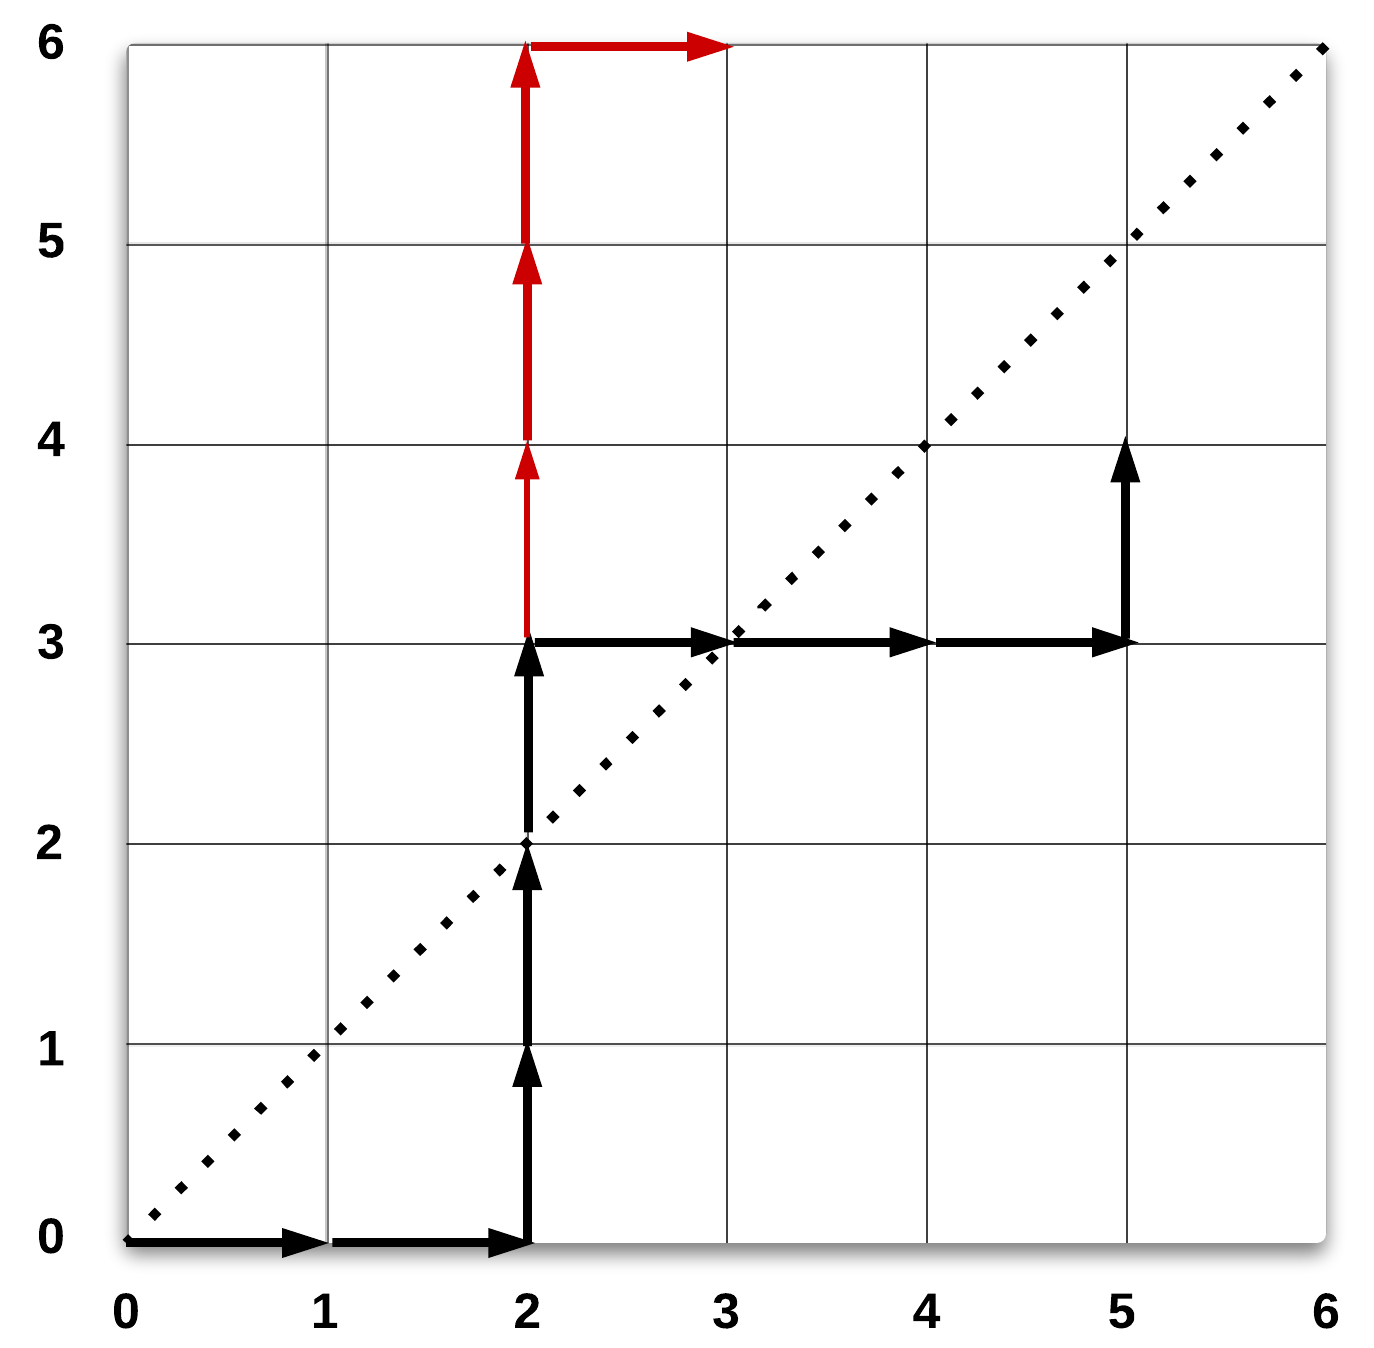
\includegraphics[width=10cm]{reflection.png}
\caption{TODO}
\label{fig:reflection}
\end{figure}

\end{document}